\begin{frame}
\centering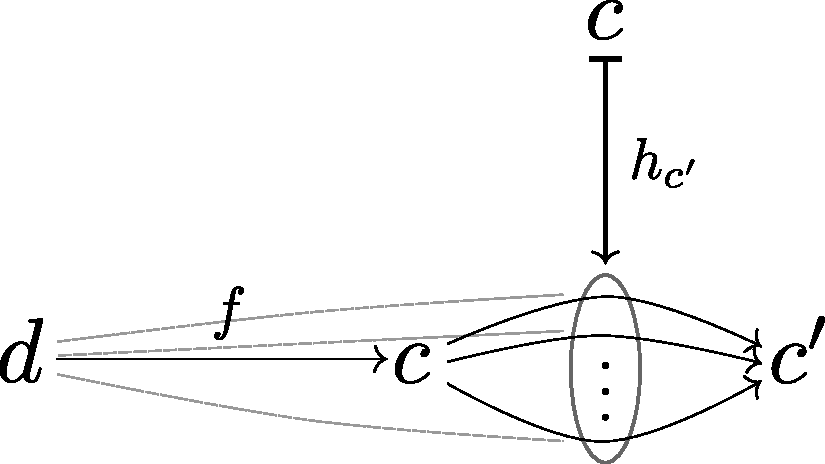
\includegraphics[width=0.7\framewidth]{fig/hom.pdf}

The presheaf represented by $c' \in \Ob(\cC)$ is $h_{c'} : \cC^{opp} \rightarrow \textit{Sets}$. It sends objects to the set of morphisms in which they are the domain object with codomain $c'$ and morphisms $f:d \rightarrow c \in \Mor{\cC}$ to set functions $h_{c'} \circ f: \Mor_{\cC}(c,c') \rightarrow \Mor_{\cC}(d,c')$ via pre-composition.
\end{frame}